\begin{homeworkProblem}
    Consider an \(n \times n\) chessboard (the figure below shows an example 
    with \(n = 8\)).

    \begin{center}
    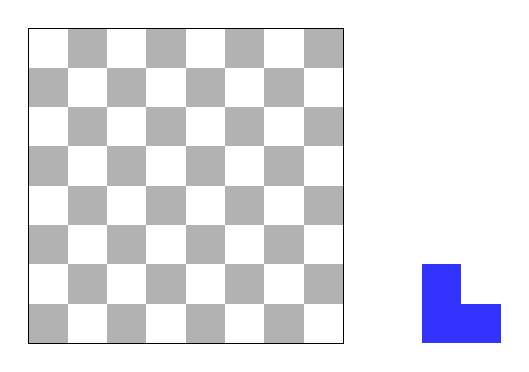
\begin{tikzpicture}[scale=0.5]
        \foreach \x in {0,...,7} {
            \foreach \y in {0,...,7} {
                \pgfmathsetmacro{\shade}{mod(\x+\y,2) == 0 ? "gray!60" : "white"}
                \fill[\shade] (\x,\y) rectangle (\x+1,\y+1);
            }
        }
        \draw (0,0) rectangle (8,8);
        
        \begin{scope}[xshift=10cm, yshift=0cm]
            \fill[blue!80] (0,0) rectangle (1,1);
            \fill[blue!80] (0,1) rectangle (1,2);
            \fill[blue!80] (1,0) rectangle (2,1);
            \draw[blue!80, line width=0.5pt] (1,0) -- (1,1);
            \draw[blue!80, line width=0.5pt] (0,1) -- (1,1);
        \end{scope}
    \end{tikzpicture}
    \end{center}

    Show that if \(n\) is a power of 2 it is possible to cover the board with 
    L-shaped trominoes (consisting of three squares each, shown in blue) so 
    that all but one of the squares on the board is covered.
    \\

    \solution

    \begin{proof}
        Below is an inductive proof on $m$ to show 
        that it is possible to cover the board with L-shaped trominoes so that 
        all but one of the squares on the board is covered.  

        \begin{itemize}
            \item \textbf{Base case:} When $m = 1$, remove any square from the
                $2^m \times 2^m$ square to reveal where the tromino will cover the
                rest of the board.
            \item \textbf{Inductive hypothesis:} Assume that for all $1 \leq m 
                \leq k$ that it is possible to cover 
                the board with L-shaped trominoes so that all but one of the 
                squares on the board is covered. 
            \item \textbf{Inductive step:} For $m = k + 1$, consider the 
                $2^{k + 1} \times 2^{k + 1}$ board as four $2^k \times 2^k$ 
                boards combined together, with each making up one quadrant of
                the larger board. It is possible to remove one square at random
                from this larger board, and the removed square will lie in one
                of the quadrants. By placing a tromino over the center of this
                larger board such that it covers those quadrants without the 
                removed square this effectively renders each quadrant as a 
                $2^k \times 2^k$ board with one square missing. By the 
                inductive hypothesis, it's the case that these can be covered
                with L-shaped trominoes so that all but one of the squares on
                the board is missing.
        \end{itemize}

        Therefore, the entire $2^{k + 1} \times 2^{k + 1}$ board can be tiled 
        with L-shaped trominoes such that all but one square on the board is 
        covered. By induction, this proves the claim for all $n \geq 1$ that
        are powers of 2. 
    \end{proof}

\end{homeworkProblem}
